\chapter{Let's \go to the Ball}
\label{dance}
\newcommand{\mail}{\q{mail}\xspace}
\newcommand{\phemail}{\q{phemail}\xspace}
\lettrine[nindent=0.1em]{I}{n previous centuries} balls were very formal affairs. Apart from the uncomfortable clothes, there were strict protocols about who could dance with whom. Ladies would keep track of their conquests with dance cards -- each dance of the evening would be listed and would be annotated with the lucky gentleman with whom she had agreed to partner that dance.
\begin{figure}
\centerline{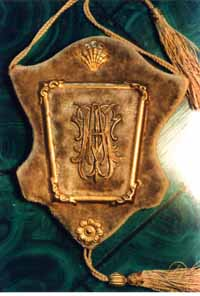
\includegraphics{dcard}}
\caption{\label{dance:card}A 19$^{th}$ Century Hungarian Dance Card}
\end{figure}

In this chapter we will look at a simulated Ball, or at least the dance negotiation part of the Ball. In our simulation we have \mail dancers and \phemail dancers; the \q{mail}s attempt to \emph{mark the card} of as many \phemail{}s as possible. Each \phemail has a preassigned number of slots in her dance card.
\begin{aside}
This is not a very realistic simulation. For one thing, many of the potential partners will already be known to each other; and also in a real Ball there are a fixed number of dance slots and each dancer has the potential to fill dance every dance.
\end{aside}
In order that dance partners can be found, we will have a directory that acts as a general kind of notice board: \phemail{}s publish a description of themselves in the directory and \mail{}s search the directory for potential partners. 

Each \mail agent has the same task -- to find \phemail{}s and to attempt to reserve a dance with them -- as many as possible. Each \phemail agent responds to requests for a dance and either grants it, or, if their dance card is already full, given the suitor a \q{rainCheck}.

Our simulation starts with a fixed number of \mail and \phemail agents, and will stop when all negotiations are complete.

\section{A negotiation protocol}
\label{dance:proto}

One way in which our simulation will be somewhat accurate is in the fact that the various dancers -- both \mail and \phemail -- will be acting as autonomous processes or threads. In order for a successful agreement to have a dance, there needs to be a negotiation between the two dancers. In our simulation, this negotiation is carried out by exchanging messages.

\subsection{Message communication in \go}
\label{dance:mbox}

\index{message communication}
\index{go.mbox@\q{go.mbox} package}
\go has a standard package -- \q{go.mbox} -- that permits threads to send and receive messages. Message communication is a high-level robust way of establishing \emph{coordination} between different threads or processes. It is, in practice, much easier to manage than using the \q{sync}hronized access to shared resources that we saw in Chapter~\ref{directory}.

\go's message communication is based on the \q{mailbox[]} and the \q{dropbox[]} abstractions. The \q{mailbox[]} is used by a thread to read messages that have been sent to it; and the \q{dropbox[]} is used by threads to send messages to its linked \q{mailbox[]}. This model is intended to be a \emph{multiple writers, single reader} communications model -- once the \q{mailbox} is created, its \q{dropbox}es can be distributed to any number of other threads of activity.

\begin{aside}
In principle, it is not required that a given \q{mailbox[]} has just one type of \q{dropbox[]} -- there could be a rich variety of \q{dropbox}es; each targeted at a different mode of message transport. However, \go's standard \q{go.mbox} package only supports a single kind of message communication: oriented towards exchanging messages between threads in a single invocation of the \go engine.
\end{aside}

\index{dropbox@\q{dropbox[]} type}
The interface for a \q{dropbox[]} is straightforward: it has a single main method -- \q{post} -- that permits messages to be delivered to its \q{mailbox[]}. Program~\vref{dance:dropbox} gives the type interface to the standard \q{dropbox[]}.
\begin{program}
\vspace{0.5ex}
\begin{alltt}
dropbox[M] \impl \{ post:[M]* \}.
\end{alltt}
\vspace{-2ex}
\caption{The standard \q{dropbox} type interface}
\label{dance:dropbox}
\end{program}
Notice also that the \q{dropbox[]} type is \emph{polymorphic}. It is polymorphic in the type of the message. Each message communication channel can handle messages of a single type. \go's message communication is strongly typed, just like other aspects of the language.

\index{mailbox@\q{mailbox[]} type}
The interface that a thread has for \emph{reading} messages is encapsulated in the \q{mailbox[]} type interface, shown in Program~\vref{dance:mailbox}. Reading messages is inherently more complex than sending them, and this interface reflects that.
\begin{program}
\vspace{0.5ex}
\begin{alltt}
mailbox[M] \impl \{
  next:[M]*. nextW:[M,number]*. pending:[]\{\}.
  msg:[M]*. msgW:[M,number]*. dropbox:[]=>dropbox[M]
\}.
\end{alltt}
\vspace{-2ex}
\caption{The standard \q{mailbox} type interface}
\label{dance:mailbox}
\end{program}

There are two ways of reading messages from a \q{mailbox}: we can read each message as it comes in -- using the \q{next} action -- or we can \emph{search} the \q{mailbox} for matching messages -- using the \q{msg} action -- which also \emph{blocks} should there be no matching message. Both the \q{msg} and the \q{next} have \emph{timeout} versions -- \q{msgW} and \q{nextW} -- that will only block for a certain time, after that they \q{raise} a \q{timedout} exception.

We find that, for many applications, the \q{msg} oriented approach is often easier to understand and leads to fewer complications; so that is how we shall proceed.

\subsection{Negotiation messages}
\label{dance:message}
\index{negotiation between agents}
In order for the \mail and \phemail agents to understand each other there has to be agreement on the messages communicated. Establishing an algebraic type is an excellent way of defining the messages that flow in a conversation -- especially since \q{mailbox[]}es and \q{dropbox[]}es are themselves typed with the type of the messages that they convey.

In general, \firstterm{conversation}{a conversation is a sequence of messages that occur between two (or more) message exchanging agents.}s are two-way; it is good practice to have two types: one for each \emph{direction} in the conversation (unless, of course, the messages in a conversation can go in either direction). This leads to a style where each conversation has two \q{mailbox/dropbox} pairs -- one pair for each direction in the conversation.

In our Ball simulation, \mail agents propose to \phemail agents, and the latter respond with yeah or nay; so we shall use two types -- as seen in program~\vref{dance:type} -- to reflect the conversations from the different perspectives of the two kinds of agent.
\begin{program}
\vspace{0.5ex}
\begin{alltt}
mailProto::=shallWe(symbol,dropbox[phemailProto]).

phemailProto::=whyNot(symbol,dropbox[mailProto]) | 
                 rainCheck(symbol,dropbox[mailProto]).
\end{alltt}
\vspace{-2ex}
\caption{The message types in the \q{dance} protocol}
\label{dance:type}
\end{program}
The \q{mailProto} type -- used by the \mail agent to propose to a \phemail agent -- has just a single constructor -- \q{shallWe}. This message is used to initiate a proposal dance.

\begin{figure}
\centering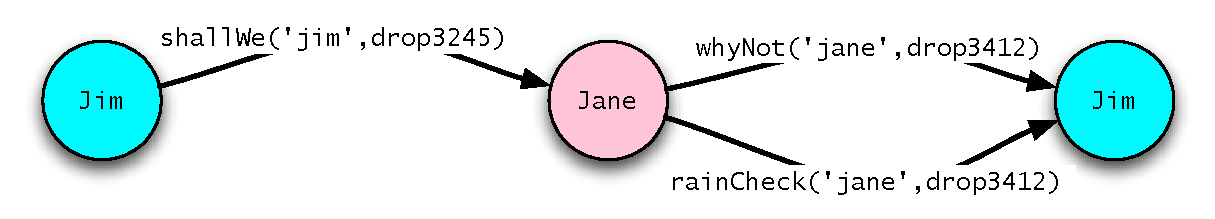
\includegraphics[width=\textwidth]{protocol}
\caption{\label{dance:protocol}A dance negotiation}
\end{figure}

Since our \mail agents don't express a preference for a particular dance, the \q{shallWe} constructor has just two arguments -- a \q{symbol} which is used simply for human readable tracing and a \q{dropbox[]}. The \q{dropbox} will be used by the \phemail agent to reply to the \mail agent. This is a familiar pattern in message-based communication: messages include in them the means of replying.

When a \mail agent sends a \q{shallWe} message to a potential partner, it will execute the \q{post} action on the \q{dropbox} belonging to the \phemail:
\begin{alltt}
\ldots;P.post(shallWe('jim',jimDropBox));\ldots
\end{alltt}
We shall see below how a \mail agent uses the directory to acquire a \phemail's \q{dropbox}; of course \q{jimDropBox} is its own \q{dropbox} -- which every agent should have easy access to.

To \emph{receive} the \q{shallWe} message, the \phemail agent executes a \q{msg} action, using its \q{mailbox}:
\begin{alltt}
\ldots;ourBox.msg(shallWe(Who,Rep));\ldots
\end{alltt}
A successful completion of this action would result in the \q{Who} and \q{Rep} variables being bound to the name of the proposer and its \q{dropbox}. Below, we shall see how the \phemail deals with the message.

There are two constructors in the \q{phemailProto} type -- the \q{whyNot} and the \q{rainCheck} constructors. The former is used by a \phemail when accepting a proposition and the \q{rainCheck} is used when rejecting it.

These constructors follow the same pattern as the \q{shallWe} constructor; but as the potential conversations between Ballroom agents are very short the true role of the \q{dropbox[]} argument in the \q{whyNot} and \q{rainCheck} messages is slightly different: to allow the \mail to \emph{confirm} that the reply message to its \q{shallWe} proposal is from the expected \phemail. Of course, there are other ways of doing this -- such as using a randomly generated number as a key.


In addition to the \q{mailProto} and \q{phemailProto} types, it is convenient to have two \q{attVal} classes for encapsulating the \q{dropbox[]}es of the two kinds of dancer:
\begin{alltt}
locM:[dropbox[mailProto]]\conarrow{}attVal.
locM(_)<=thing.

locF:[dropbox[phemailProto]]\conarrow{}attVal.
locF(_)<=thing.
\end{alltt}
We will use these constructors to publish and search the ballroom's directory for appropriate partners.


\begin{aside}
A more elaborate conversation protocol would almost certainly have a richer collection of message types. In addition, each message would carry more information. One immediate thought for a suitable extension would be the name of the particular dance being proposed and/or disposed. For example, a \mail agent might propose the first Waltz, and the \phemail might respond with an acceptance for the second Polka. However, we leave aside such elaborations in this example.
\end{aside}

\section{A \mail agent}
\label{dance:mail}

The task of the \mail agent is to locate as many \phemail agents as possible and to propose to dance with them. We might express this as the iteration:
\begin{alltt}
P in Phemails *> propose(P)
\end{alltt}
except that it may be useful to collect information about the \phemail agents it encounters (after all, negotiation is but the first step in the dance). So, the heart of our \mail dancer is the computation of the bounded set expression:
\begin{alltt}
\{ P .. (P::propose(P)) in Phemails \}
\end{alltt}
where \q{propose} is a predicate that is satisfied for every successful proposal to a \phemail agent. Recall that an expression such as:
\begin{alltt}
P::propose(P)
\end{alltt}
is a \emph{guarded pattern}, and, in this case, denotes a \q{P} which is a member of the list \q{Phemails} for which \q{propose} is satisfied.

In a successful negotiation, the \mail agent must first send a \q{shallWe} message to the \phemail, and must receive a \q{whyNot} message in reply. Of course, it is possible that the reply is a \q{rainCheck}, in which case there will be no dance.

This is an instance where the success of a predicate -- \q{propose} -- depends on the results of a sequence of \emph{actions}. \go has mechanisms for relating actions to expressions and predicates: we saw a use of the \q{valof/valis} combination in Program~\vref{directory:package}. For predicates we have the \q{action} predicate condition: an \q{action\{\}} condition wraps an action sequence as a way of satisfying a predicate.

\subsection{A \mail proposal}

\index{action@\q{action} query}
To satisfy a \q{propose}, we need to send a message and receive a reply; we can do this with the relation definition:
\begin{alltt}
propose:[dropbox[mailProto]]\{\}.
propose(P) :- action\{
    P.post(shallWe(ourName,ourDrop));
    ourBox.msg(Reply);
    istrue whyNot(H,\_).=Reply
  \}.
\end{alltt}
where we are assuming some auxiliary definitions: \q{ourName} and \q{ourDrop} are the symbolic names of this \mail dancer and its \q{dropbox} respectively and \q{ourBox} is its \q{mailbox}. The argument to \q{propose} is directly a \q{dropbox}.

The form:
\begin{alltt}
action\{ \ldots istrue \emph{Condition} \ldots\}
\end{alltt}
is the query analogue of the \q{valof}/\q{valis} expression condition. The action
\begin{alltt}
istrue whyNot(H,\_).=reply
\end{alltt}
determines the truth value associated with the \q{action} itself. If the query condition
\index{match query}
\index{operator!.=@\q{.=}}
\begin{alltt}
whyNot(H,\_).=reply
\end{alltt}
is satisfied, then the truth value will be \q{true} and the \q{action} will succeed also.

This query condition represents a \emph{match} of the pattern \q{whyNot(H,\_)} against the variable \q{Reply}. This is the same kind of matching that is used in the head of an action rule against the arguments of the action -- and in the head of an equation against the function call. In this case the match succeeds if \q{Reply} is \emph{already} bound to a value of the form \q{whyNot(H,\_)} -- i.e., the match may not bind \q{Reply} -- although it may bind variables on the left hand side of the condition. The second variable in the \q{whyNot(H,\_)} pattern is \emph{anonymous} and no-one cares what its values is anyway, but the first is used to collect names of dance partners.

\subsection{A \mail class}
\index{mail@\q{mail} class}
When we build our ballroom, we will want the various dancer agents to execute in parallel -- to reflect their autonomous nature. We expect our dance agents to carry some \emph{state} -- in particular a record of the dance partners that they have agreed to dance with. On the other hand, that state is essentially \emph{private} to the dancers and should not be unnecessarily exposed. Although \q{mail} and \q{phemail} dancers are quite different internally, from a top-level perspective they should be managed in the same way within the simulation.

To regularize this, we propose a \q{dancer} interface that the top-level simulation uses to \q{spawn} and otherwise control the dancers and each dancer agent -- \mail and \phemail -- will be expected to implement that interface:
\begin{alltt}
dancer \typearrow{} \{ start:[]*. report:[]=>string \}
\end{alltt}
The \q{start} action will be invoked when the dancer agent is expected to start executing -- we should of course also have a \q{stop} action. The \q{report} function is there to permit the top-level simulation to request a report on the status of each dancer.

In Program~\vref{dancer:mail} we wrap up the \mail agent in a class body -- that implements this \q{dancer} interface type -- including some of the auxiliary definitions hinted at above. Since the \mail is a stateful entity we use the \sconarrow{} class constructor in establishing the type of the \mail class.

Note that \q{explode} -- it is used in the \q{report} function -- is a standard library function that is used here to convert the \q{Name} \q{symbol} into a \q{string}.

\begin{program}[bt]
\vspace{0.5ex}
\begin{alltt}
mail:[symbol]\sconarrow{}dancer.
mail(ourName)..\{
  ourBox:mailbox[phemailProto] = mailbox.
  ourDrop:dropbox[phemailProto] = ourBox.dropbox().
  partners:list[symbol] := [].

  propose:[dropbox[mailProto],symbol]\{\}.
  propose(P,H) :- action\{
     P.post(shallWe(ourName,ourDrop));
     ourBox.msg(Reply);
     istrue whyNot(H,_).=Reply
   \}.

  Phemails:[]=>list[dropbox[mailProto]].
  Phemails() => \{ locOf(A) .. A in 
     dir.find([at('gender',aG(female))],['loc']) \}.

  locOf:[list[attr]]=>dropbox[mailProto].
  locOf(A) :: at('loc',locM(P)) in A => P.

  start() -> 
     partners := \{ H..(P::propose(P,H)) in Phemails() \}.

  report() => explode(Name)<>" with "<>partners.show().
\}
\end{alltt}
\vspace{-2ex}
\caption{A \mail dancer class}
\label{dancer:mail}
\end{program}

The \q{Phemails} function queries the shared directory to locate descriptions that have a \q{'gender'} attribute of \q{female}. The \q{dropbox} of the \phemail agent is extracted from the description using the \q{locOf} auxiliary function.

\subsubsection{Assignment in a class}
\index{class!assignment in}
The \q{start} action procedure has an \emph{assignment} within it:
\begin{alltt}
partners := \{ P..(P::propose(P)) in Phemails() \}
\end{alltt}
Assignment is permitted for special re-assignable variables declared in a class body; in the case of the \q{partners} variable its declaration was:
\begin{alltt}
partners:list[symbol] := [].
\end{alltt}
\go supports reassignable variables, but with some restrictions: their values must be ground -- they may not have any unbound variables within their value -- and they are \emph{private} to a class body or package. In particular, they may not be re-assigned outside the context that they are declared. For variables declared in a class body, that means that only rule programs defined in the same class body may modify their values. Finally, only stateful classes -- introduced with the \sconarrow{} class constructor type -- are permitted to define constants and variables in their class body.

These restrictions are there partly to permit reasonable implementations and partly to control the implications of having a re-assignable variable. Ensuring that only programs defined in the same scope may modify variables means that program analysis is that much simpler. It also means that it is not possible for a programmer to subtly change the semantics of a variable defined in a super class.

Program~\vref{dancer:mail} also has a \emph{constant} definition within it:
\begin{alltt}
  ourDrop:dropbox[phemailProto] = ourBox.dropbox().
\end{alltt}
\q{ourDrop} is a constant because, once its value is established, it cannot be overwritten with a new value -- unlike variables. 

An object constant like this is established every time an instance of the \mail class is created. Thus every time we evaluate the constructor expression \q{mail(\emph{Name})} a new \q{ourBox} is also created, and a new copy of \q{ourDrop} established.

\section{A \phemail agent}
\label{dance:phemail}

\index{phemail@\phemail class}
The \phemail agent is the counterpart of the \mail agent; its heart is an action that waits for \q{shallWe} messages from proposing \mail agents and responds to those messages. This is preceded by an initialization phase in which the \phemail posts a description of itself with the shared directory.

\index{directory!registering with}
The simplest description consists of the \q{name} of the agent, its \q{gender} and, critically, the \q{dropbox} that the \mail agents can use to contact the \phemail:
\begin{alltt}
init() -> dir.register([at('name',aS(Name)),
                        at('gender',aG(female)),
                        at('loc',locM(ourDrop))]).
\end{alltt}
Note that although the \phemail agent publishes its name, the \mail agent is not actually interested in the name. This is a common scenario: agents that publish descriptions of themselves will often \emph{over-describe} themselves -- it is difficult to predict the actual uses of services ahead of time. The flexibility of the attribute/value style of descriptions makes this over-description harmless.

\begin{program}[h]
\vspace{0.5ex}
\begin{alltt}
phemail:[symbol,integer]\sconarrow{}dancer.
phemail(Nme,Limit)..\{
  ourBox:mailbox[mailProto] = mailbox.
  drop:dropbox[mailProto] = ourBox.dropbox().
  partners:list[symbol] := [].

  init() -> dir.register([at('name',aS(Nme)),
                          at('gender',aG(female)),
                          at('loc',locM(drop))])
  
  accepting:[integer]*.
  accepting(Count)::Count>0 ->
    ourBox.msg(shallWe(Who,Rep));
    Rep.post(whyNot(Nme,drop));
    partners := [Who,..partners];
    accepting(Count-1).
  accepting(0) -> rejecting().

  rejecting:[]*.
  rejecting() -> ourBox.msg(shallWe(_,Reply));
    Reply.post(rainCheck(Nme,ourBox));
    rejecting().

  start() -> init(); accepting(Limit).

  report() => explode(Nme)<>" with "<>partners.show().
\}
\end{alltt}
\vspace{-2ex}
\caption{A \phemail dancer class}
\label{dancer:phemail}
\end{program}

If we assume that each \phemail has a predefined limit of how many partners it can accept then the main loop of the agent can be captured in two action procedures \q{accepting} for when the \phemail is accepting proposals and \q{rejecting} for when it is not. This is achieved in Program~\vref{dancer:phemail} by using two recursive action procedures -- \q{accepting} and \q{rejecting}. When in the \q{accepting} procedure, the dancer is potentially accepting new proposals; when there is no more room, the \q{accepting} action procedure calls the \q{rejecting} procedure -- which never accepts any proposals.

The \q{accepting}/\q{rejecting} pair of action procedures make, in effect, a simple state machine. State machines are a common technique for constructing simple agents; although more complex behaviors require more sophisticated approaches.

\section{The Ballroom}
\label{dance:ballroom}
The final piece of our simulation is the ballroom itself; or the top-level driver of the simulation. At the top-level we model each \q{dancer} as a separate thread of activity, as well as another thread for the \q{directory}. 

The main phases of the simulation driver are an initialization phase -- where the different agents are created and \q{spawn}ed off -- a waiting phase and the final reporting phase.

Managing a \q{spawn}ed off activity can be challenging: we need to be able to coordinate with it and to potentially kill it off or wait for it to terminate. 

\index{expression!spawn@\q{spawn}}
We have seen that \q{spawn} is an action; it is also an \emph{expression}. The value returned by a \q{spawn} expression is the thread identifier of the new activity -- of type \q{thread}. This value can be used to determine the state of the thread, or otherwise manage it: the \q{kill} function terminates a thread and the \q{waitfor} action procedure suspends until the thread has terminated (naturally or not).

For our purposes we will \q{spawn} a number of \mail threads of activity and \phemail threads. The latter do not have a natural termination as a \phemail cannot know if there are more \mail{}s to propose. On the other hand, a \mail agent, as we have written it in program~\vref{dance:mail}, does terminate once it has proposed to all the \phemail{}s it finds from the directory.

We can use this termination as a way of deciding when the simulation should enter its final reporting phase:
\begin{alltt}
\ldots ( M in \emph{MailThreads} *> waitfor(M)); \ldots
\end{alltt}
\index{forall!action}
\index{operator!*>@\q{*>}}
This uses the \emph{forall} operator -- \q{*>} -- as an action; we have already seen its use as a predicate condition in program~\vref{directory:directory}. In this case we iterate over the known \mail threads, waiting for each to finish. When they are all ended we assume that the simulation has stabilized.

\begin{program}[tb]
\vspace{0.5ex}
\begin{alltt}
main(_) ->
  stdout.outLine("Starting...");
  Phems = [ phemail('jill',1),phemail('jane',2),
            phemail('joan',3),phemail('jenny',4)];
  (F in Phems *> spawn\{F.start()\});
  Mails = \{ mail(N) .. N in ['fred','jim','peter',
                              'alfred','john'] \};
  (M in \{ spawn\{ MM.start()\} .. MM in Mails\}*>waitfor(M));
  stdout.outLine("Reporting...phems...");
  (F in Phems *> stdout.outLine(F.report()));
  stdout.outLine("Reporting...mayls...");
  (M in Mails *> stdout.outLine(M.report())).
\end{alltt}
\vspace{-2ex}
\caption{Top-level of Ballroom simulation}
\label{dance:main}
\end{program}

A complete top-level main program is shown in program~\vref{dance:main}; inevitably, this \q{main} program has something of the character of a sequential script: starting programs off, waiting for them to finish, collecting information. A sample run of our ballroom simulation looks like:
\begin{alltt}
Starting...
Reporting...phems...
jill with ['fred']
jane with ['jim','fred']
joan with ['peter','jim','fred']
jenny with ['alfred','peter','jim','fred']
Reporting...mayls...
fred with ['jill','jane','joan','jenny']
jim with ['jane','joan','jenny']
peter with ['joan','jenny']
alfred with ['jenny']
john with []
\end{alltt}

\section{Summing up}
So far, we have seen a little of the style and programming power of the programming language \go. The ballroom simulation is a fairly complex program that would take many times as much space in some other programming languages. Yet, for the most part, it is also quite an elegant program and we are not over-burdened with a lot of minor details.


